\documentclass{beamer}
\usepackage{xcolor}
%\usepackage{fontspec}
%\setmainfont{Georgia}
%\usepackage[T1]{fontenc}
\usepackage{winfonts}
\usepackage[backend=bibtex]{biblatex}
\renewcommand{\sfdefault}{georgia}

\bibliography{report}

%%%%%%%%%%%%%%
% Soton colourscheme

%primary palette:           RED    GREEN  BLUE
\definecolor{sotonblu}{rgb}{.00392 .26275 .34902} % soton blue
\definecolor{sotongrn}{rgb}{.00000 .44706 .45882} % soton green
\definecolor{sotoncya}{rgb}{.03922 .58824 .66275} % soton cyan
\definecolor{sotongry}{rgb}{.19608 .23922 .26275} % soton grey
\definecolor{sotonbei}{rgb}{.59216 .61961 .27059} % soton beige
\definecolor{sotonmet}{rgb}{.73333 .73333 .73333} % soton metal

%some secondary colors:
\definecolor{sotonyel}{rgb}{.99999 .70196 .00000} % soton yellow
\definecolor{sotonora}{rgb}{.99608 .24314 .07843} % soton orange
\definecolor{sotonred}{rgb}{.94118 .05882 .17255} % soton red
\definecolor{sotonrus}{rgb}{.67059 .07059 .06275} % soton russet
\definecolor{sotonbrn}{rgb}{.54118 .25490 .16863} % soton brown
\definecolor{sotonpnk}{rgb}{.88627 .41176 .62353} % soton pink
\definecolor{sotonppl}{rgb}{.32549 .12157 .26667} % soton purple


\setbeamertemplate{background canvas}[vertical shading][top=sotonblu,bottom=sotoncya]
\setbeamercolor{background canvas}{bg=}
\setbeamercolor{button border}{bg=sotonblu, fg=sotonblu}
\setbeamercolor{button}{bg=sotonblu, fg=DarkRed}

\setbeamercolor{frametitle}{fg=sotonyel}
\setbeamercolor{alerted text}{fg=sotonyel}
\setbeamercolor{normal text}{fg=white}
\setbeamercolor{titlelike}{fg=sotonyel}
\setbeamercolor{author}{fg=white}
\setbeamercolor{date}{fg=white}
\setbeamercolor{item}{fg=white}

%%%%%%%%%%%%%%%%%%%%

\title{CDT for Next Generational Computational Modelling (NGCM):\\ High Temperature Nano-Magnetic Materials}
\author{Jonathon Waters\inst{1}}
\institute{
	\inst{1}
	Engineering and the Environment,\\
	University of Southampton,\\
	UK\\
	
	Contact: J.M.Waters@soton.ac.uk
}
\date{}

\begin{document}
\frame{\titlepage 

\includegraphics[height=1cm]{Images/sponsor-wo}\hfill
\includegraphics[height=1cm]{Images/uos_grey_large}}

\setbeamertemplate{headline}{
	\vskip25pt % horizontal line
	\vskip-21pt\hspace{2pt}\hfill
\includegraphics[height=7mm]{Images/sponsor-wo}\hspace{3.5mm}
\includegraphics[height=7mm]{Images/uos_grey_large}\hspace{3.5mm} % logo on the right
}

\setbeamertemplate{footline}{
	\vskip-8pt % horizontal line
	\hspace{12cm} \insertframenumber/\inserttotalframenumber
	\vskip4pt
}

\begin{frame}
	\frametitle{Speaker Background}
	\begin{columns}
		\column{7cm}
		\begin{itemize}
			\item{2010 - 2014: MPhys(Hons) Physics with Theoretical Physics at the University of Manchester.\newline}
			\item{Summer 2013: Worked at the Deutsches Elektronen-Synchrotron (DESY) as a member of the ATLAS project.\newline}
			\item{2014 - Present: Member of CDT in NGCM}
		\end{itemize}
		\column{5cm}
		\begin{center}
			
\includegraphics[width=3.5cm]{Images/hardhat} \vspace{2mm}
			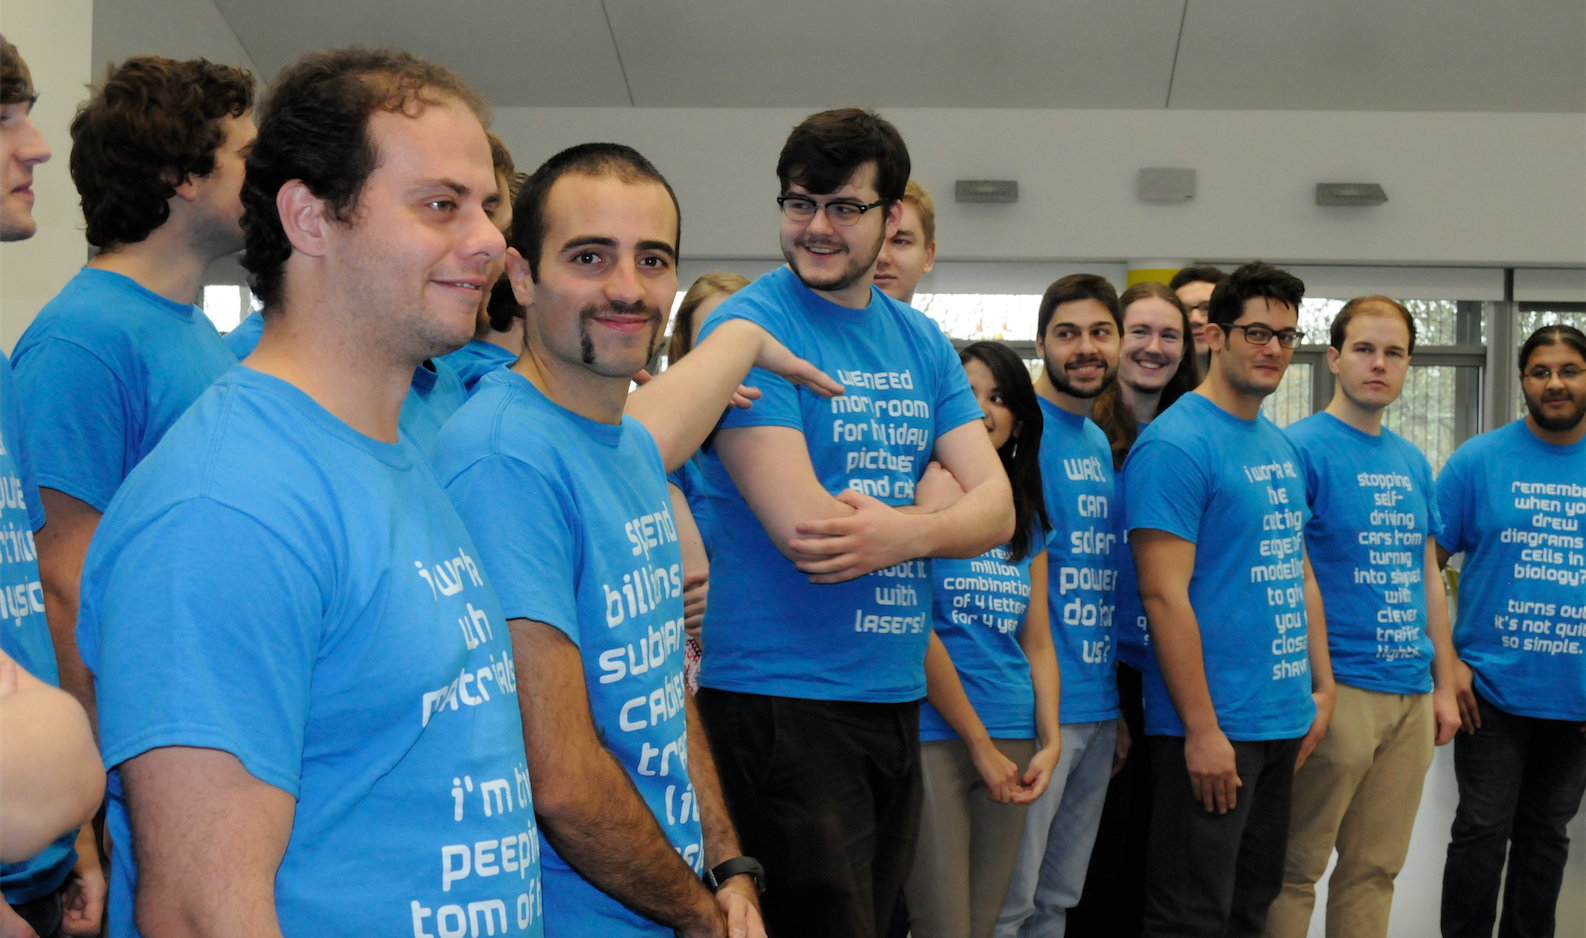
\includegraphics[width=5cm]{Images/ngcm2}
		\end{center}
	\end{columns}
\end{frame}

\begin{frame}
	\frametitle{My Research}
	
\end{frame}

\begin{frame}
	\frametitle{Applications}
	\begin{columns}
		\column{6cm}
		In HAMR\footnotemark[1]:
		\begin{itemize}
			\item{$T_C$ distribution affects the noise performance}
		\end{itemize} \vspace{5mm}
		
		\begin{center}
		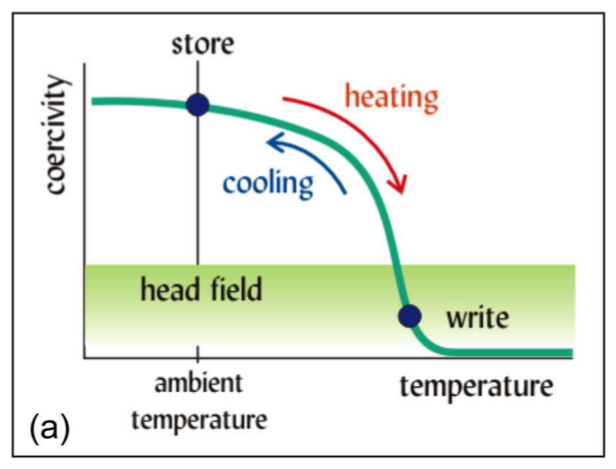
\includegraphics[width=2.9cm]{Images/coerc} \hspace{1mm}
		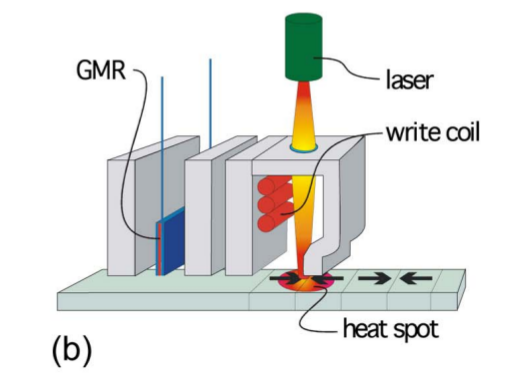
\includegraphics[width=2.9cm]{Images/laser} \\
		\tiny E. Dobisz et al. Proc IEEE 96.11, 1836 (2008)
		\end{center}
		
		\column{6cm}
		In Magnetic Hyperthermia\footnotemark[2]:
		\begin{itemize}
		\item{Low $T_C$ reduces tissue damage}
		\end{itemize}
		
		\begin{center}
		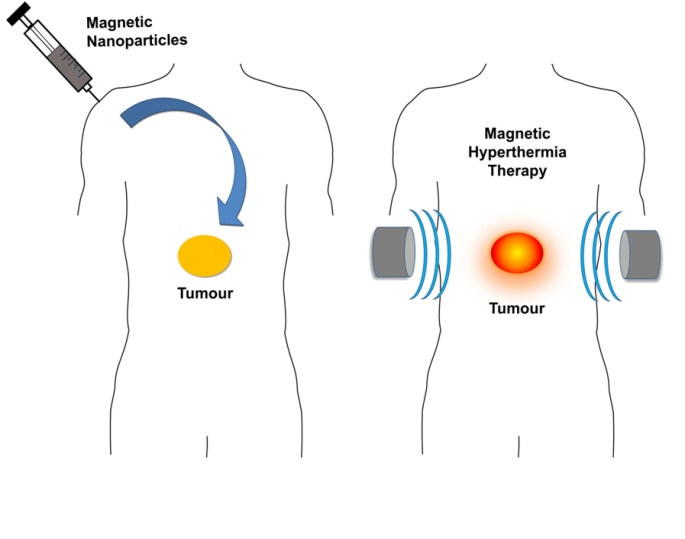
\includegraphics[width=4cm]{Images/person} \\
		\tiny \^{A}ngela Andrade et al. Coating Nanomagnetic Particles for Biomedical Applications (2011)
		\end{center}
	\end{columns}
	\footnotetext[1]{\tiny D. Weller et al. IEEE Transactions on Magnetics 50.1, 3100108 (2014)}
	\footnotetext[2]{\tiny I Apostolova et al. Solid State Communications 149.25, 986 (2009)}
\end{frame}

\begin{frame}
	\frametitle{CDT in NGCM}
	\begin{columns}
		\column{7cm}
		The CDT has helped support this project through extensive training: \vspace{2mm}
		\begin{itemize}
			\item{Learnt 4 new programming languages}
			\begin{itemize}
				\item{Python, R, Julia, C}\vspace{2mm}
			\end{itemize}
			\item{Training in High Performance Computing (HPC)}
			\begin{itemize}
				\item{OpenMP, MPI, Intel Xeon Phi, GPU programming}\vspace{2mm}
			\end{itemize}
			\item{Software development skills}
			\begin{itemize}
				\item{Version control, virtual machines, continuous integration}\vspace{2mm}
			\end{itemize}
			\item{Numerical methods, Statistics.....}
		\end{itemize}
		\column{5cm}
		\begin{center}
			
\includegraphics[height=1.25cm]{Images/julia}\\
			
\includegraphics[height=1cm]{Images/python}
			
\includegraphics[height=1cm]{Images/R} \vspace{14mm}
			
\includegraphics[height=1.5cm]{Images/intel}\hspace{0.2cm}
			
\includegraphics[height=1.5cm]{Images/nividia}
		\end{center}
	\end{columns}
\end{frame}

\begin{frame}
	\frametitle{CDT in NGCM}
	\begin{columns}
		\column{5cm}
		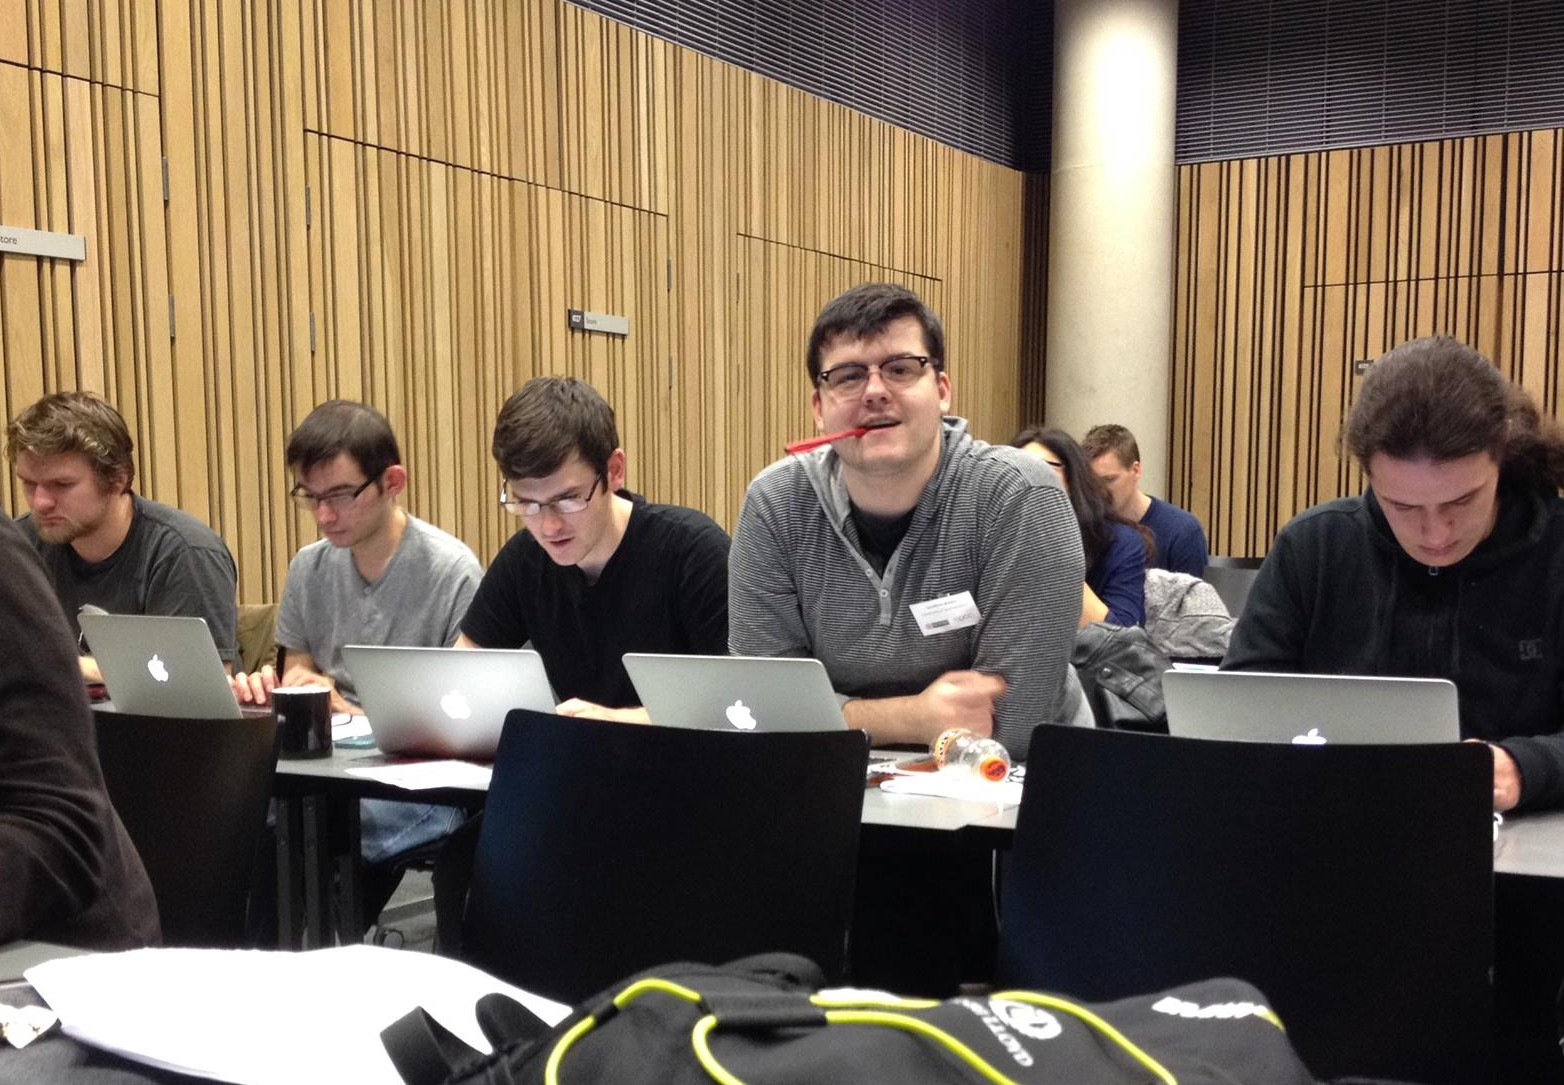
\includegraphics[width=5cm]{Images/ngcm}
		\column{7cm}
		Freedom to explore my own interests through: \newline
		\begin{itemize}
			\item{Delivering a workshop on the Julia language}\newline
			\item{Individual research projects during the first year and summer}\newline
			\item{Organising and attending the NGCM Summer Academy}
		\end{itemize}
	\end{columns}
\end{frame}

\begin{frame}
	\begin{center}
		\huge{Thank you for listening}\vspace{8mm}
		
		\large{Contact: J.M.Waters@soton.ac.uk}
	\end{center}
\end{frame}

\begin{frame}
	\frametitle{Defining Finite Sized $T_C$}
	\begin{columns}
		\column{6cm}
		\begin{center}
		Correlation length $\propto |T-T_C^b|^{-\nu}$ \\ \vspace{3mm}
		Grain size, $D \propto |T_C(D)-T_C^b|^{-\nu}$ \\ \vspace{3mm}
		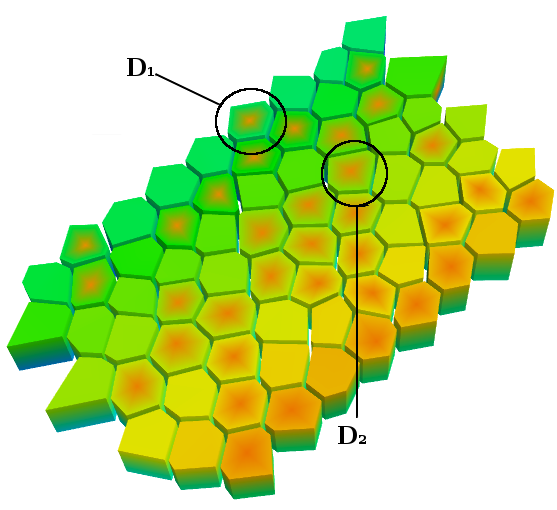
\includegraphics[width=5cm]{Images/grains2}
		\end{center}
		\column{6cm}
		\begin{center}
		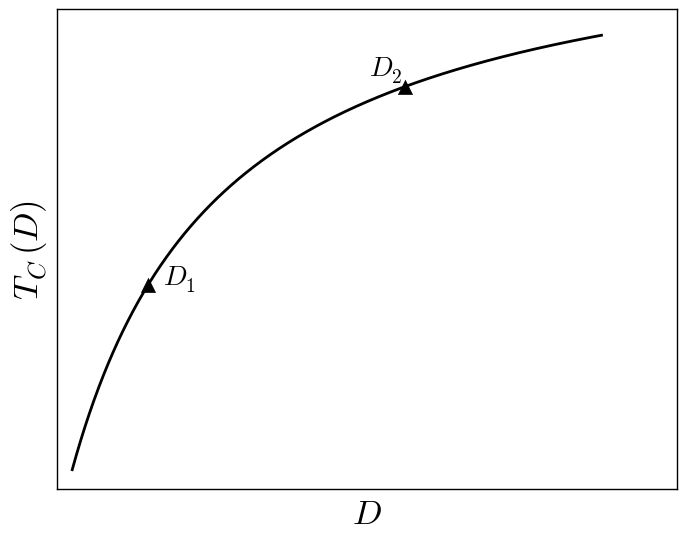
\includegraphics[width=5cm]{Images/TcD}
		\vspace{4mm}
		Distribution in $D$ leads to distribution in $T_C$
		$$
		f_D(D) \Longrightarrow f_{T_C}(T_C)
		$$
		\end{center}
	\end{columns}
\end{frame}

\begin{frame}
	\frametitle{Currently Used Methods}
	\vspace{4mm}
	\begin{itemize}
		\item{Explicit measurement of individual grains.\footnotemark[3]}
		\begin{itemize}
			\item{Switching temperature is measured by a laser system set up}
			\item{This is related to $T_C$}
		\end{itemize}
		\vspace{4mm}
		\item{Identification from macroscale measurements\footnotemark[4]}
		\begin{itemize}
			\item{Single measurement with magnetometer}
			\item{Integral measure}
			\item{But uses bulk relations}
		\end{itemize}
	\end{itemize}	
	\footnotetext[3]{\tiny S. Pisana et al. IEEE Transactions on Magnetics 51.4, 1 (2015)}
	\footnotetext[4]{\tiny A. Berger et al. J. Appl. Phys. 91.10, 8393 (2002)}
\end{frame}

\begin{frame}
	\frametitle{Objectives}
	\begin{itemize}
		\item{Develop a universal method to identify the $T_C$ distribution which incorporates the finite size effects of the individual grains\newline}
		\item{Test the method against a well quantified benchmark (2D Ising system) in order to verify it's effectiveness for different distributions.\newline}
	\end{itemize}
\end{frame}

\begin{frame}
	\frametitle{Our Method}
	\begin{columns}
	\column{8cm}
	\small{
	\newline
	Magnetisation for Ensemble of Grains:
	$$
	M(T) = M_0\int_0^\infty D^{d} m(D,T) f_D(D) dD
	$$
	Single Grain Magnetisation:
	$$
	m(D,T) \propto D^{-\beta/\nu} \mu \left(D^{1/\nu}\frac{T-T_C^b}{T_C^b}\right)
	$$
	Change of Variables:
	$$
	D = d_0\left(\frac{T_C^b - T_C(D)}{T_C^b}\right)^{-\nu} 
	$$
	Final Result:
	$$
	M(T) = M_0^*\int_0^{T_C^b} t^{-d\nu +\beta} \mu\left(\frac{T-T_C^b}{t}\right) f_t(t) dt
	$$}
	\column{4cm}
	\begin{center}
	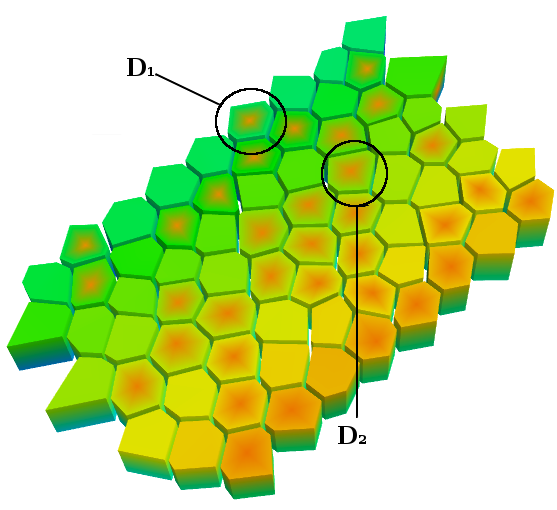
\includegraphics[width=2.5cm]{Images/grains2}	
	
	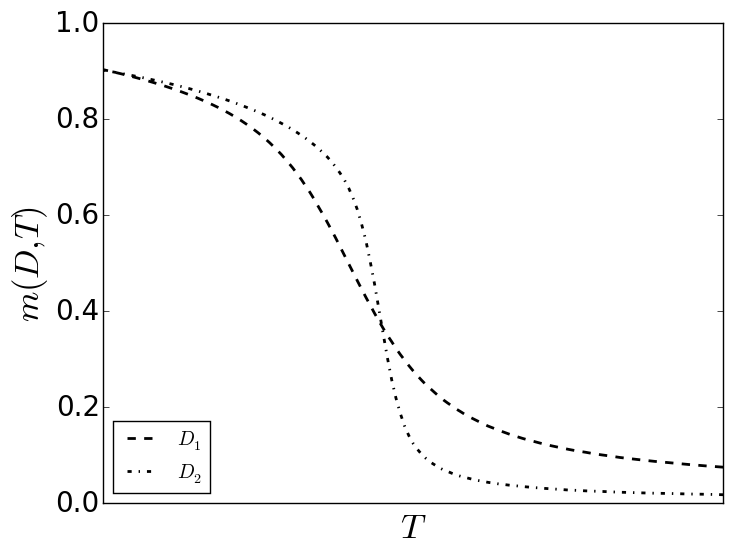
\includegraphics[width=3.25cm]{Images/Ds_noinset}
	
	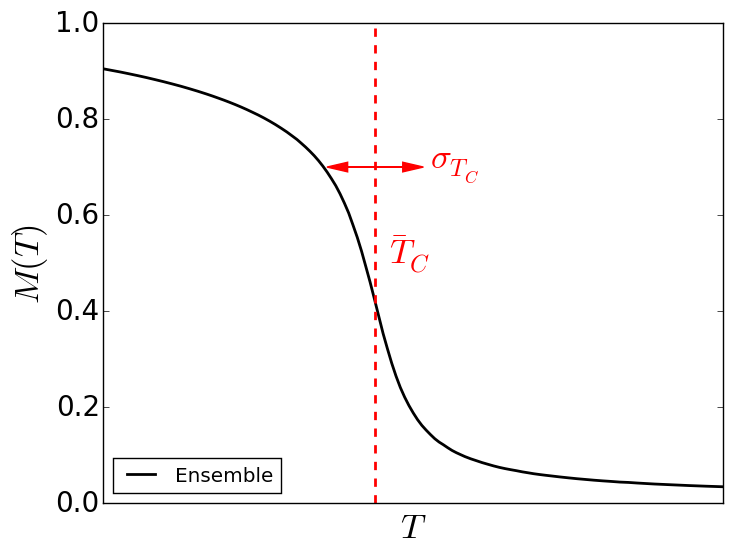
\includegraphics[width=3.25cm]{Images/Aggregate}
	\end{center}
	\end{columns}
\end{frame}

\begin{frame}
	\frametitle{Finding $f_t$}
		
	\begin{center}
	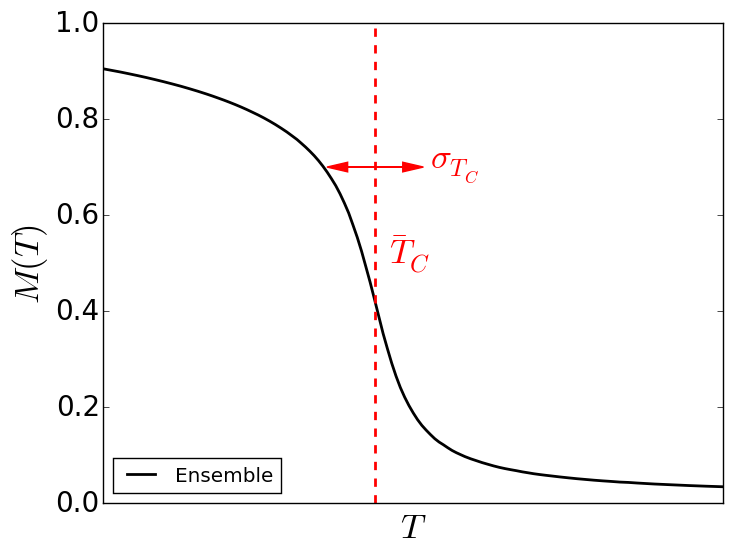
\includegraphics[width=4cm]{Images/Aggregate} \hspace{3mm}
	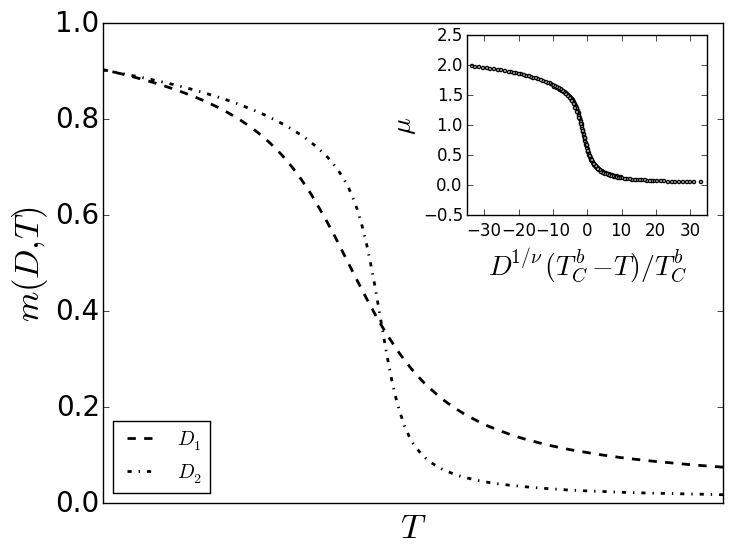
\includegraphics[width=4cm]{Images/Ds}
	
	$$
	M(T) = M_0^*\int_0^{T_C^b} t^{-d\nu +\beta} \mu\left(\frac{T-T_C^b}{t}\right) f_t(t) dt
	$$
	
	\begin{itemize}
		\item{$M(T)$: To be fitted}
		\item{$d$, $\nu$, $\beta$, $\mu$: Known information about the material}
		\item{$T_C^b$: May be known, otherwise taken from fit}
		\item{$M_0^*$, $f_t$ [ $\bar{t}$, $\sigma_t$ ]: Taken from the fit}
	\end{itemize}
	
	$$
	\bar{T}_C = T_C^b - \bar{t} \quad \quad \sigma_{T_C} = \sigma_t
	$$
	
	\end{center}
\end{frame}

\begin{frame}
	\frametitle{Test Case: 2D Ising Model}
	\begin{columns}
	\column{7cm}
		\small{
		$$
		M(T) = M_0^*\int_0^{T_C^b} t^{-d\nu +\beta} \mu\left(\frac{T-T_C^b}{t}\right) f_t(t) dt
		$$}
		Used 2D Ising model as a benchmark:
		\begin{itemize}
			\item{Simulated using Monte Carlo}
			\item{Analytical results for $\beta$, $\nu$, $T_C^b$}
			\begin{itemize}
				\item{$\beta = 1.25$}
				\item{$\nu=1$}
				\item{$T_C^b \approx 2.269$}
			\end{itemize}
		\end{itemize} \vspace{4mm}
		
		Tested against different $f_D$:
		\begin{itemize}
			\item{All mean $\bar{D}=100$}
			\item{Standard deviation $\sigma_D=10, 20, 30 ,40$}
		\end{itemize}
	\column{5cm}
		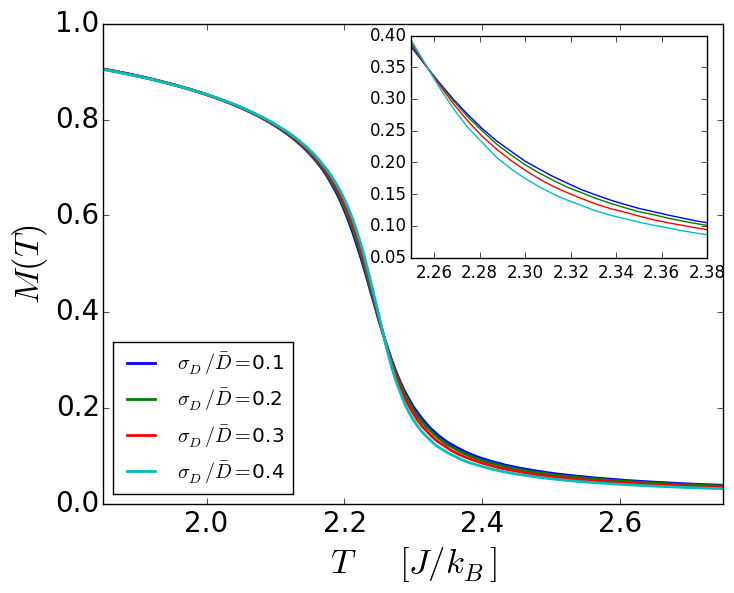
\includegraphics[width=4.5cm]{Images/distros}
		
		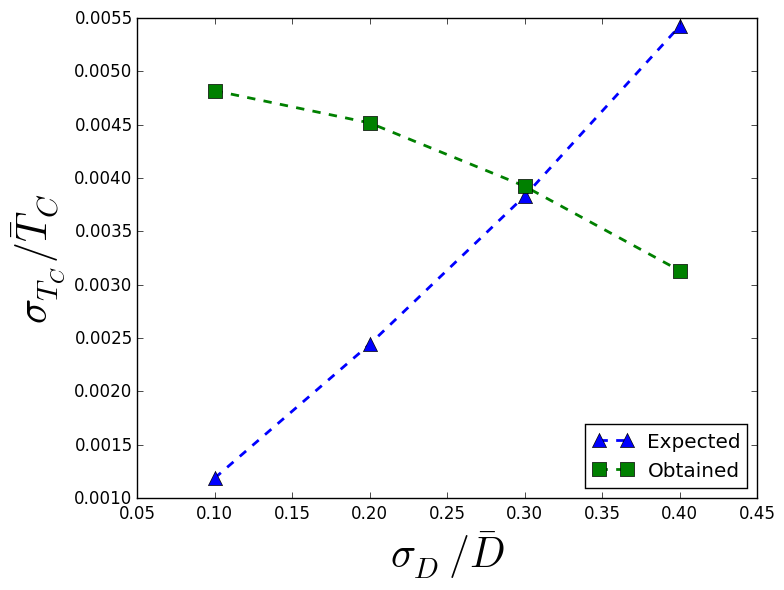
\includegraphics[width=4.5cm]{Images/unconst}
	\end{columns}
\end{frame}

\begin{frame}
	\frametitle{Test Case: 2D Ising Model}
	\begin{columns}
	\column{7cm}
		Introduce constraint\footnotemark[5]:
		$$
		\Rightarrow \sigma_{T_C}^2 = (T_C^b - \bar{T}_C)^2\left(\left(1 + \frac{\sigma_D^2}{\bar{D}^2}\right)^{1/\nu^2}-1\right)
		$$
		
		In the Ising model:
		$$
		\nu = 1
		$$
		$$
		\Rightarrow \sigma_{T_C} = (T_C^b - \bar{T}_C)\frac{\sigma_D}{\bar{D}}
		$$
		\begin{center}\vspace{2mm}
		
		Fitted results far better!
		\end{center}
	\column{5cm}
		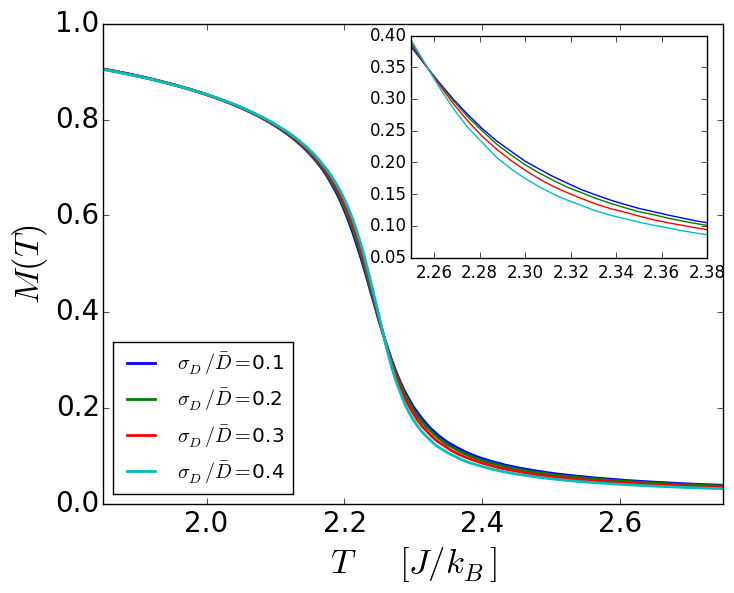
\includegraphics[width=4.5cm]{Images/distros}
		
		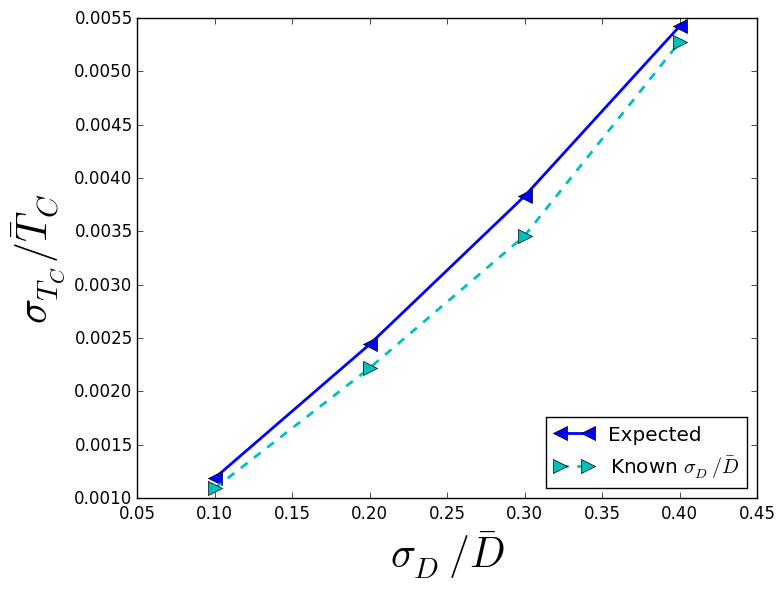
\includegraphics[width=4.5cm]{Images/constr}
	\end{columns}
	\footnotetext[5]{\tiny O. Hovorka et al. Appl. Phys. Letters 101.5, 052406 (2012)}
\end{frame}

\begin{frame}
	\frametitle{Conclusions}
	\small{
	\begin{itemize}
		\item{Universal method to find size dependent $T_C$ distribution based upon fitting ensemble magnetisation:}
		$$
		M(T) = M_0^*\int_0^{T_C^b} t^{-d\nu +\beta} \mu\left(\frac{T-T_C^b}{t}\right) f_t(t) dt
		$$
		\item{Successfully tested against 2D Ising model (without a loss in generality) and found a strong parameter correlation which can be solved by the constraint:}
		$$
		\sigma_{T_C}^2 = (T_C^b - \bar{T}_C)^2\left(\left(1 + \frac{\sigma_D^2}{\bar{D}^2}\right)^{1/\nu^2}-1\right)
		$$
		\item{Future work may find this insignificant in other systems. e.g. Heisenerg model, FePt Hamiltonian e.c.t.}
	\end{itemize}}
\end{frame}

\end{document}